\begin{figure*}[ht!]
\centering
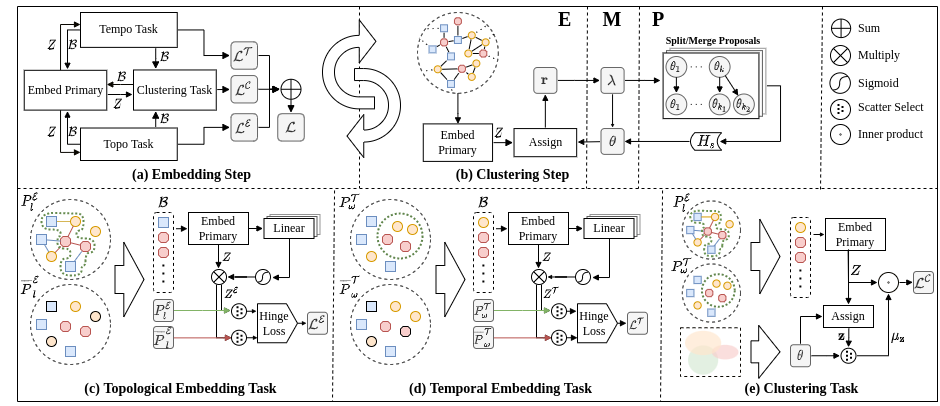
\includegraphics[width=\textwidth]{resources/framework.png}
\caption{Overview of the MGTCOM framework.
(a) In the embedding step primary embeddings are used in auxiliary tasks to construct the multi-objective loss. 
(b) Clustering step updates clustering by alternating between Expectation (\textbf{E}), Maximization (\textbf{M}), and Proposal (\textbf{P}) steps.
(c) In the topological (topo) embedding task, random walk sampling and feature-wise attention minimize inter-node proximity.
(d) In the temporal (tempo) embedding task, ballroom walk sampling and feature-wise attention minimize proximity between temporally related nodes.
(e) Clustering task adds community awareness to the embeddings by minimizing proximity between nodes within the same cluster.
}
\label{fig:framework}
\end{figure*}